%% Global Finance Journal submission draft
%% Compile: pdflatex gfj_main (twice)
%% All numbers generated by Analysis/scripts/* from Analysis/processed/event_firm_panel.csv
\documentclass[review,12pt,authoryear]{elsarticle}

\usepackage{amsmath,amssymb}
\usepackage{booktabs}
\usepackage{graphicx}
\usepackage{threeparttable}
\usepackage[flushleft]{threeparttablex}
\usepackage{multirow}
\graphicspath{{figures/}}

\newcommand{\pp}{\,pp}
\journal{Global Finance Journal}

\begin{document}

\begin{frontmatter}

\title{Compute Complementarity and Competitive Spillovers:\\
The Stock Market Pricing of Large Language Model Releases}

\author[sdu]{Zhuo Chen\corref{cor1}}
\ead{zhuochen@sdu.edu.cn}
\author[sdu]{Ruishuang Lu}
\cortext[cor1]{Corresponding author.}
\affiliation[sdu]{organization={Center for Economic Research, Shandong University},
city={Jinan}, country={China}}

\begin{abstract}
How do stock markets price the release of large language models? We construct a
reproducible event-study pipeline covering 124 day-verified model releases from
2022 to 2026 and an exogenously selected universe of Nasdaq-100 and PHLX
Semiconductor index constituents, with ecosystem positions assigned by
double-blind coding. Three results emerge. First, upstream hardware suppliers
earn 1.7 percentage points and direct competitors 1.6 percentage points of
cumulative abnormal return over twenty trading days after a release; downstream
deployers show a precisely estimated zero. Second, the hardware premium is a
late-sample phenomenon: absent through 2024, it reaches 4.3 percentage points in
2025--2026 and 4.6 percentage points around reasoning-model releases,
consistent with markets learning to treat releases as compute-demand news.
Third, model capability itself is not positively priced---anticipated flagship
releases earn no capability premium---and open-weight releases do not erode the
hardware premium. Earlier results built on non-reproducible measurements
reverse under our pipeline.
\end{abstract}

\begin{keyword}
Large language models \sep Event study \sep AI supply chain \sep
Compute complementarity \sep Market efficiency
\\ \textit{JEL codes}: G14 \sep O33 \sep G12
\end{keyword}

\end{frontmatter}

%% ============================================================
\section{Introduction}
%% ============================================================

On January 27, 2025, one week after the Chinese startup DeepSeek posted the
weights of its reasoning model R1 on GitHub, NVIDIA lost 17\% of its market
value in a single session---the largest one-day dollar loss for any stock in
U.S. history. The episode is routinely cited as evidence that artificial
intelligence model releases redistribute value along the AI supply chain, with
efficient open-source models threatening the rents of compute suppliers. Single
events, however, make treacherous evidence. Across the 124 verified model
releases we study, the DeepSeek episode sits in the far left tail of the
distribution of hardware-supplier returns: on average, upstream hardware firms
\emph{gain} after model releases, and they gain most after precisely the kind
of reasoning-model releases that R1 exemplifies.

This paper asks how equity markets price large language model (LLM) releases,
using the cross-section of ecosystem positions---hardware suppliers, cloud
providers, downstream integrators and deployers, competitors, investors, and
publishers---to identify which economic channel the market capitalizes. We
assemble 124 release events between April 2022 and March 2026 whose
announcement dates we verify to the day against first-party sources, and we
measure abnormal returns for 108 index-member firms whose ecosystem positions
are assigned under a double-blind coding protocol (Cohen's $\kappa$ between
0.84 and 1.00 across dimensions). Because the firm universe consists of
Nasdaq-100 and PHLX Semiconductor constituents, selection into the sample is
exogenous to any hypothesis about AI exposure, and the thirty-one constituents
with no classifiable relationship to AI provide a within-event control group.

Three findings emerge. First, releases redistribute value toward the upstream
and toward rivals. Over a $[0,+20]$ trading-day window, hardware suppliers earn
a cumulative abnormal return (CAR) of 1.66\pp{} ($p=0.012$; 1.79\pp{} under a
Fama--French three-factor benchmark, $p=0.007$) and direct competitors earn
1.61\pp{} ($p=0.013$), relative to unrelated firms in the same event window and
conditional on firm characteristics. Downstream deployers---firms that use AI
as a tool inside a non-AI business---show a CAR of $-0.07$\pp{} with a standard
error of 0.25\pp{}: a precisely estimated zero that rules out effects more
negative than $-0.6$\pp{}. The same contrast holds in trading activity.
Hardware suppliers display abnormal volume of 0.12 standard deviations on the
announcement day itself ($p<0.01$), while deployers show neither abnormal
returns nor abnormal volume; cloud providers trade heavily (abnormal volume
0.29 standard deviations, $p<0.01$) without directional price consensus.

Second, the hardware premium is not a constant feature of the AI era; it
\emph{formed} during the sample. Around LLM releases in 2022--2024 the
within-event hardware coefficient is statistically zero. In 2025--2026 it is
4.28\pp{} ($p<0.001$), and around reasoning-model releases it reaches
4.61\pp{}. The window profile in the late sample shows textbook gradual
incorporation: significant by day two, accumulating monotonically through day
twenty, orthogonal to the pre-event drift. Even the scope of the pricing rule
expanded: releases of media-generation models moved hardware stocks
\emph{negatively} in 2024 ($-4.7$\pp{}, $p=0.03$) but positively in 2025--2026
($+3.5$\pp{}, $p=0.02$), as video generation itself became compute-intensive.
We interpret this as the market updating its model of what an LLM release
means: from application news to compute-demand news.

Third, what the market prices is position, not capability. Using Artificial
Analysis benchmark scores as a direct measure of model capability, we find no
positive capability premium: among closed-source releases the capability slope
is significantly \emph{negative} ($-0.06$\pp{} per index point, $p=0.02$),
consistent with flagship releases being priced in advance of the announcement;
among unrelated firms the slope is zero, as a placebo requires. Capability
matters only as an amplifier of position: the interaction of capability with
the hardware indicator is positive. Relatedly, open-weight releases do not
attenuate the hardware premium (interaction $p=0.90$)---the market, unlike the
commentary that followed the DeepSeek episode, does not price open weights as a
threat to compute rents on average.

The magnitudes are economically material. A 4.3\pp{} within-event spread over
twenty trading days, applied to hardware constituents whose market
capitalizations range from tens of billions to several trillion dollars,
represents tens of billions of dollars of relative revaluation per flagship
release. At the portfolio level, a calendar-time strategy long the thirty
hardware suppliers and short the forty downstream firms earns a three-factor
alpha of about 24\% annualized over the sample ($p=0.054$); because event
windows blanket 56\% of trading days, we read the portfolio as scale rather
than identification and place the identifying weight on within-event
comparisons.

Our identification strategy rests on within-event cross-sectional comparisons.
Event fixed effects absorb everything common to an event window, including
market-wide AI sentiment; position indicators are pre-assigned at the
(firm, developer) level under a codebook fixed before estimation; and the
thirty-one zero-relationship constituents anchor the counterfactual. The
design survives an extensive battery: the hardware and competitor premia are
significant in 16--17 of 20 specifications spanning benchmarks (S\&P~500,
Nasdaq-100, SOX, three-factor), windows, winsorization, date-confidence
subsamples, exclusion of multi-component events, and event fixed effects, and
they are insensitive to release-time corrections (we verify announcement
timestamps for 55 events; shifting all events by one trading day leaves the
$[0,+20]$ estimate unchanged at 4.68\pp{} in the late sample).

A final contribution is methodological. An earlier version of this project,
built---as much of the emerging literature is---on hand-collected events and
externally supplied abnormal returns, found the opposite headline results: a
significant \emph{negative} effect for downstream firms and a significant
\emph{positive} capability premium for closed-source releases. Neither
survives the reproducible pipeline. A forensic decomposition shows why: 17 of
24 matched legacy events carried announcement dates 2 to 120 days off
first-party evidence; the legacy ``$[0,+20]$'' returns behave as if accumulated
over roughly $[-10,+20]$; and under \emph{any} date--window combination the
legacy returns correlate with assumption-free market-adjusted returns at no
more than 0.55, against 0.93 for our measure. Since results this fragile can
steer an entire narrative, we report the full specification curve and release
the pipeline.

We contribute to three literatures. Event studies of technology announcements
document value effects for innovators and rivals
\citep{chaney1991,chen2005,kogan2017}; we extend the object of study from the
announcing firm to the full ecosystem cross-section, and we show the pricing
rule itself changed over a four-year window. Work on AI and asset prices ranks
firms by exposure to generative AI \citep{eisfeldt2023,babina2024}; our
position taxonomy unbundles ``exposure'' into channels with opposite
predictions and shows that the compute-complementarity channel, not average
exposure, carries the pricing. Studies of information transfer along supply
chains \citep{lang1992,cohen2008,gofman2020,barrot2016} predict heterogeneous
spillovers from economic linkages; the positive competitor spillover we find
indicates that contagion-type industry information dominates the competitive
effect \citep{lang1992} in a fast-growing technology sector. Methodologically,
we join the literature on specification fragility and researcher degrees of
freedom \citep{simonsohn2020,brodeur2020,mitton2022} with a concrete case in
which measurement reconstruction reverses published-style results.

Section~\ref{sec:lit} develops hypotheses. Section~\ref{sec:data} describes
the pipeline, the coding protocol, and the measurement audit.
Section~\ref{sec:results} presents baseline results,
Section~\ref{sec:formation} the formation of compute pricing,
Section~\ref{sec:capability} the capability tests, and
Section~\ref{sec:robust} robustness. Section~\ref{sec:conclusion} concludes.

%% ============================================================
\section{Related literature and hypotheses}\label{sec:lit}
%% ============================================================

\subsection{The economics of an LLM release}

A frontier model release is informative about cash flows at several layers of
a vertical supply chain at once. At the top sit the model developers
themselves---some listed (Alphabet, Meta, Microsoft, Amazon), most private
(OpenAI, Anthropic, xAI, DeepSeek). One layer down are the compute
complements: designers of accelerators and high-bandwidth memory, the
foundries and equipment makers behind them, and the interconnect, power, and
server vendors that turn chips into clusters. Cloud platforms rent this
capacity and increasingly resell frontier models through hosted interfaces.
Downstream, integrators build products whose core input is model capability,
while deployers use AI as a tool inside businesses whose revenue does not
depend on it.

Which layer a release is news for depends on how models turn into costs and
revenues. Training is a one-off, capitalized expenditure; inference is a
recurring marginal cost that scales with usage. Two developments during our
sample window shifted the expected compute intensity of the industry from
the first margin to the second. Reasoning models---beginning with releases
in late 2024 and accelerating through 2025---consume orders of magnitude
more inference compute per query by trading test-time computation for
accuracy, and their adoption converts model quality improvements into
recurring demand for accelerators and data-center capacity. Video-generation
models underwent the same transition in 2025, when high-resolution synthesis
became a mass-market inference workload. If investors understand this
mapping, a capability release is derived-demand news for the upstream; if
they instead read releases as application or displacement news, the pricing
should concentrate downstream. The cross-section of positions around
releases therefore identifies which economic model of AI the market holds
at a point in time---and letting the coefficients vary over time reveals
whether that model itself changed.

\subsection{Predictions}

Classical event-study logic holds that publicly datable, salient events allow
abnormal returns to measure revisions in expected cash flows
\citep{fama1969,brown1985,mackinlay1997,kothari2007}. Product introductions
carry such information for the announcer and, with opposite sign, for rivals
\citep{chaney1991,hendricks1997,chen2005,sorescu2007}. An LLM release differs
from a conventional product introduction in that it simultaneously shifts the
expected cash flows of firms across an entire vertical ecosystem, as just
described.

Two families of predictions follow. The \emph{complementarity} view treats a
frontier release as news about derived demand for training and inference
inputs: more capable models require and monetize more compute, benefiting
upstream asset owners \citep{acemoglu2012,gofman2020}. The
\emph{substitution} view emphasizes that as foundation models absorb
capabilities, the differentiation space of downstream products narrows
\citep{bommasani2021,zhu2018}, depressing deployer and integrator values.
Industry information transfer adds a third margin: a release may signal
sector-wide growth (contagion) or a rival's competitive loss
\citep{lang1992}. Finally, appropriability logic suggests open-weight releases
should weaken any premium built on proprietary compute demand
\citep{teece1986,lerner2002,solaiman2023}.

We test four hypotheses.

\textbf{H1} (\emph{position heterogeneity}): abnormal returns around LLM
releases differ systematically across ecosystem positions within the same
event.

\textbf{H2} (\emph{direction}): upstream compute complements earn positive
abnormal returns; downstream deployers earn negative abnormal returns. (We
find the first half supported and the second half rejected in favor of a
precise zero.)

\textbf{H3} (\emph{open-source moderation}): the upstream premium is weaker
for open-weight releases. (Not supported.)

\textbf{H4} (\emph{formation}): if the premium reflects compute-demand news,
its strength should increase as the reasoning paradigm shifts compute from
one-off training toward recurring inference; the pricing rule should
strengthen over time and be strongest around reasoning-model releases.
(Supported, including an expansion of the rule's scope to compute-intensive
media models.)

%% ============================================================
\section{Data and measurement}\label{sec:data}
%% ============================================================

\subsection{Release events}\label{sec:events}

The event universe intersects two independent public sources: the AI Timeline
project, a curated chronology of AI model releases, and Artificial Analysis
(AA), a third-party benchmarking platform. An event enters the candidate set
only if the released model is covered by AA, which screens out announcements
too minor to be benchmarked. Identity matching between the two sources is
resolved by a scored matcher with all manual decisions recorded in an
auditable decision table; family releases announced together are merged into
one event. The pipeline yields 134 events, of which 125 have day-level release
dates verified against first-party sources (vendor engineering blogs, release
notes, model repositories, or archived first captures); the nine events
without verifiable day-level dates are dropped. One further event whose
identity is inconsistent across sources is flagged and excluded from the main
sample, leaving 124 events: 3 from 2022, 8 from 2023, 45 from 2024, 59 from
2025, and 9 from 2026. Eighty-seven events are language-model releases with AA
intelligence scores; thirty-five are media-generation releases with AA Elo
scores; two are speech models without comparable scores.

Date verification matters. For each event we record the source and confidence
of the date; known pitfalls include vendor pages that render UTC timestamps
(shifting evening announcements to the next calendar day) and Chinese vendors'
Beijing-date pages (which typically coincide with the correct U.S. reaction
day). For 55 events we further recover intraday release times from page
metadata or archived first captures; only two events have positive evidence of
after-hours release. Section~\ref{sec:robust} shows results are insensitive
to any feasible re-dating.

\subsection{Firm universe and ecosystem positions}\label{sec:positions}

The firm universe is the union of Nasdaq-100 and PHLX Semiconductor (SOX)
constituents at collection date: 108 firms, of which 101 Nasdaq-100 members
form the main sample and SOX-only members are used in robustness. Index
membership makes selection exogenous to AI exposure and supplies a natural
control group: thirty-one constituents (consumer staples, utilities, health
care) have no classifiable relationship to any model developer.

Each (firm, developer) pair---108 firms $\times$ 25 developers---is coded on
eight dimensions following a fixed codebook: upstream hardware (R1), upstream
cloud (R2), downstream integrator (R3), downstream deployer (R4), downstream
enabler (R5), competitor (R6), investor (F1), and owner/publisher (F2). Two
coders worked double-blind; agreement was 99.0\% across the 21,600 cell
decisions, with dimension-level Cohen's $\kappa$ between 0.839 and 1.000;
disagreements were adjudicated against the codebook with all decisions logged.
Event-level indicators take the union over the event's developers. Event
attributes (open-weight status, reasoning, modality, family release) were
likewise double-coded ($\kappa$ 0.917--1.000).

\subsection{Abnormal returns and abnormal volume}\label{sec:car}

Daily total returns for all firms and benchmarks come from adjusted closing
prices (January 2021 to April 2026). Abnormal returns follow the market model
with the S\&P~500 as market proxy, estimated over trading days $[-200,-10]$
relative to the event day (minimum 120 observations); we cumulate over
$[0,+w]$ for $w \in \{0,1,2,3,5,10,15,20\}$ and a pre-event window $[-10,-2]$.
We deliberately avoid a Nasdaq-100 benchmark for the main results because
sample firms are its constituents; QQQ- and SOX-benchmark CARs and
Fama--French three-factor CARs are computed for robustness. Firm controls
(log assets, book-to-market, prior-year momentum, estimation-window
volatility) are matched under a strict as-of rule: only statements whose
fiscal period ended at least 45 days before the event date are used. Negative
book equity (buyback-driven, 711 firm-events) is flagged and excluded from the
book-to-market control rather than entered as a negative ratio.

Abnormal volume is the standardized abnormal log volume: the deviation of
daily log volume from its $[-200,-10]$ mean, scaled by its estimation-window
standard deviation, averaged over the event window.

\subsection{A measurement audit}\label{sec:audit}

An earlier vintage of this project used hand-collected events and externally
computed abnormal returns, a practice common in the emerging AI event-study
literature. Its two headline results---significantly negative deployer CARs
and a significantly positive capability premium for closed-source
releases---\emph{reverse} under the pipeline of
Sections~\ref{sec:events}--\ref{sec:car}. A three-layer forensic audit locates
the difference entirely in measurement rather than in sample composition:
restricting the legacy panel to the firms and events shared with the new
sample leaves the legacy results intact, while recomputing returns for the
identical cells eliminates them.

The three layers are: (i) \emph{dates}---17 of 24 matched legacy events carry
announcement dates that differ from first-party evidence by 2 to 120 days;
(ii) \emph{windows}---a scan across all window definitions shows the legacy
``day $[0,+1]$'' return series is most consistent with a $[-1,+1]$ window and
the legacy ``$[0,+20]$'' series with roughly $[-10,+20]$, i.e., post-event
windows contaminated by pre-event returns; and (iii) an \emph{unattributable
residual}---under the best date--window combination the legacy series
correlates with assumption-free market-adjusted returns (raw return minus
S\&P~500 return, no estimation) at 0.55, against 0.93 for our series on the
same cells. A two-by-two swap test on identical firm--event cells shows that
replacing the capability regressor (old versus new benchmark vintages) leaves
the legacy result intact, while replacing the return measure eliminates it.
We conclude the legacy results were artifacts of compound measurement error,
and we flag this as a caution for a literature in which event dates are
frequently taken from secondary aggregators
\citep{simonsohn2020,brodeur2020,mitton2022}.

\subsection{Descriptive statistics}

Table~\ref{tab:desc} summarizes the panel: 12,112 firm-event observations
(124 events $\times$ 101 firms, less late listings without full estimation
windows). Twenty-five percent of firm-events carry a hardware relationship,
5\% cloud, 12\% integrator, 20\% deployer, 5\% competitor; 26\% of
observations belong to zero-relationship control firms.

\begin{table}[t!]
\centering
\begin{threeparttable}
\caption{Sample composition and descriptive statistics}\label{tab:desc}
\small
\begin{tabular}{lrrrr}
\toprule
 & \multicolumn{4}{c}{Events by year and type} \\
\cmidrule(lr){2-5}
 & 2022--23 & 2024 & 2025 & 2026 \\
\midrule
All events            & 11  & 45  & 59  & 9 \\
\quad LLM (AA intelligence score)   & 5   & 32  & 44  & 6\tnote{a} \\
\quad Media generation (AA Elo)     & 6   & 12  & 14  & 3 \\
\quad Reasoning-model events        & 0   & 4   & 31  & 6 \\
\quad Open-weight events            & 4   & 20  & 20  & 3 \\
\midrule
 & \multicolumn{4}{c}{Firm-event panel (main sample)} \\
\cmidrule(lr){2-5}
 & Obs. & Mean $\beta$ & Mean CAR$[0,20]$ & SD \\
\midrule
Upstream hardware   & 2{,}708 & 1.99 & $+2.08$\% & 12.7\% \\
Upstream cloud      & \phantom{0,}568  & 1.37 & $-0.75$\% & 9.6\% \\
Downstream integrator & 1{,}981 & 1.42 & $-0.63$\% & 11.3\% \\
Downstream deployer & 2{,}971 & 0.96 & $-0.07$\% & 9.3\% \\
Competitor          & \phantom{0,}753  & 1.24 & $-0.32$\% & 7.0\% \\
No relationship (control) & 3{,}967 & 0.68 & $-0.08$\% & 9.7\% \\
\bottomrule
\end{tabular}
\begin{tablenotes}\footnotesize
\item Notes: The main sample excludes one event with inconsistent identity
across sources. Position categories overlap (multi-label coding); the control
row counts firm-events with no positive indicator on any dimension.
\item[a] Two 2026 speech-model events carry no comparable AA score.
\end{tablenotes}
\end{threeparttable}
\end{table}

%% ============================================================
\section{Baseline results: position pricing}\label{sec:results}
%% ============================================================

\subsection{Position premia}

Table~\ref{tab:baseline} reports the baseline cross-sectional regressions of
CAR$[0,+20]$ on the seven position indicators, firm controls, and year fixed
effects, with standard errors clustered by event (CR2). Column (1) uses the
S\&P~500 market model, column (2) the three-factor model, and column (3) adds
event fixed effects, identifying purely from within-event variation.

\begin{table}[t!]
\centering
\begin{threeparttable}
\caption{Ecosystem position and cumulative abnormal returns}\label{tab:baseline}
\small
\begin{tabular}{lccc}
\toprule
Dependent variable: & (1) CAR$^{MM}[0,20]$ & (2) CAR$^{FF3}[0,20]$ & (3) CAR$^{MM}[0,20]$ \\
\midrule
Upstream hardware      & 0.0166** & 0.0179*** & 0.0154** \\
                       & (0.0065) & (0.0065)  & (0.0066) \\
Upstream cloud         & $-$0.0011 & 0.0020   & $-$0.0018 \\
                       & (0.0078) & (0.0074)  & (0.0076) \\
Downstream integrator  & $-$0.0051 & $-$0.0041 & $-$0.0053 \\
                       & (0.0049) & (0.0048)  & (0.0050) \\
Downstream deployer    & $-$0.0007 & 0.0002   & $-$0.0011 \\
                       & (0.0025) & (0.0024)  & (0.0025) \\
Competitor             & 0.0161** & 0.0159*** & 0.0158** \\
                       & (0.0064) & (0.0058)  & (0.0064) \\
Investor               & 0.0090   & 0.0145    & 0.0087 \\
                       & (0.0114) & (0.0113)  & (0.0115) \\
Owner/publisher        & 0.0152   & 0.0151    & 0.0148 \\
                       & (0.0138) & (0.0135)  & (0.0139) \\
\midrule
Firm controls          & Yes & Yes & Yes \\
Year fixed effects     & Yes & Yes & --- \\
Event fixed effects    & --- & --- & Yes \\
Observations           & 12{,}112 & 12{,}112 & 12{,}112 \\
Events                 & 124 & 124 & 124 \\
\bottomrule
\end{tabular}
\begin{tablenotes}\footnotesize
\item Notes: Firm controls are log assets, book-to-market (with a
negative-equity indicator), estimation-window volatility, and prior-year
momentum. Standard errors clustered by event (CR2) in parentheses.
*, **, *** denote 10\%, 5\%, 1\% significance.
\end{tablenotes}
\end{threeparttable}
\end{table}

Hardware suppliers earn 1.66\pp{} more than unrelated constituents over the
twenty days following a release ($p=0.012$); the estimate is 1.79\pp{} under
the three-factor benchmark and 1.54\pp{} within events. Direct competitors
earn a statistically indistinguishable premium of 1.61\pp{}. The competitor
premium is noteworthy: rivalry-based models of product announcements predict
negative wealth effects for competitors \citep{chen2005}; the positive sign
indicates that in this period an LLM release conveyed industry-level growth
information that dominated the competitive-displacement effect, the contagion
pattern of \citet{lang1992}.

The deployer coefficient is $-0.07$\pp{} with a standard error of 0.25\pp{}.
This is not an underpowered non-result: the 95\% confidence interval,
$[-0.56, +0.42]$\pp{}, excludes deployer losses larger than one third of the
hardware gain. The market did not, on average, price LLM releases as bad news
for firms that deploy AI inside conventional businesses.

The remaining positions sharpen the interpretation. Cloud providers---the
most direct resellers of model capability---show a price response of zero
(column~1: $-0.11$\pp{}, $p=0.89$), a fact we return to below because it
coexists with the largest trading response in the panel. Integrators are
mildly negative but imprecise ($-0.51$\pp{}, $p=0.30$). Investors and
owner-publishers carry positive point estimates of 0.9 and 1.5\pp{} but few
independent clusters (their positive cells concentrate in a handful of
developers), so we do not lean on them. The economically meaningful contrast
is the roughly 1.7\pp{} spread between hardware suppliers and deployers
within the same event window---firms facing the same release, the same
market conditions, and the same AI sentiment, distinguished only by where
they sit in the production chain.

Figure~\ref{fig:profile} traces the window profile. In the full sample the
hardware premium emerges at $[0,+10]$ and grows through $[0,+20]$; in the
2025--2026 subsample it is significant from $[0,+2]$ ($+0.51$\pp{}),
accumulates monotonically to $+4.28$\pp{}, and is preceded by a modest
pre-event run-up. Crucially, controlling for the firm's own pre-event CAR
leaves the post-event estimate unchanged (4.28\pp{} to 4.35\pp{}), so the
accumulation is not a continuation of pre-existing drift.

\begin{figure}[t!]
\centering
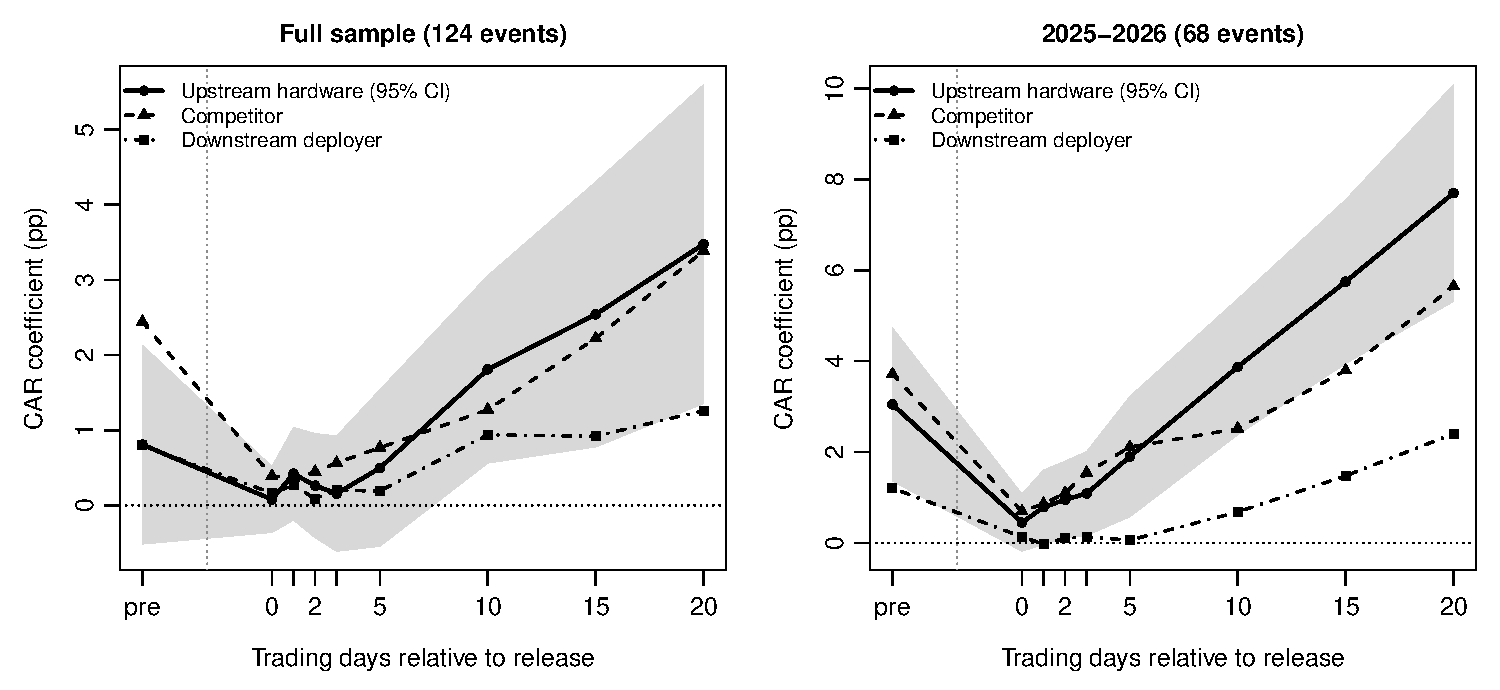
\includegraphics[width=\textwidth]{fig1_car_profile}
\caption{Cumulative abnormal returns around LLM releases by ecosystem
position. Coefficients on position indicators from window-by-window
cross-sectional regressions with firm controls and year fixed effects;
shading is the 95\% confidence band for the hardware coefficient (event-level
CR2 clustering). The leftmost point is the pre-event window $[-10,-2]$.}
\label{fig:profile}
\end{figure}

\subsection{Trading activity}

Table~\ref{tab:volume} repeats the design with standardized abnormal log
volume as the outcome. Hardware suppliers trade abnormally heavily on the
announcement day itself---0.12 standard deviations at $[0,+1]$
($p<0.01$)---including in the full sample where the same-horizon price
response is still indistinguishable from zero. Attention arrives immediately;
directional consensus forms over days. Deployers show no abnormal volume at
any horizon ($p=0.74$ at $[0,+1]$): their zero price response reflects genuine
irrelevance rather than offsetting disagreement. Cloud providers are the
mirror image---the largest abnormal volume in the panel (0.29 standard
deviations at $[0,+1]$; 0.44 in 2025--2026) with no directional price
response, the signature of repricing activity without consensus. The cloud
volume anomaly extends into the pre-event window ($0.20$ standard deviations
over $[-10,-2]$, $p<10^{-5}$; $0.31$ in 2025--2026): cloud names attract
heavy trading before and at announcements without ever settling on a
direction. In disagreement models, volume without price movement is the
fingerprint of investors interpreting the same public signal with different
priors \citep{kandel1995}; cloud platforms fit naturally, since a frontier
release is simultaneously good news for their compute-rental business and
bad news for their own model ambitions and gross margins. No other position
shows pre-event abnormal volume---in particular, the hardware pre-event
price run-up documented above is \emph{not} accompanied by trading
intensity. The three downstream fates thus separate cleanly: hardware is
priced with consensus, cloud is traded without consensus, and deployers are
ignored on both margins.

\begin{table}[t!]
\centering
\begin{threeparttable}
\caption{Abnormal trading volume around releases}\label{tab:volume}
\small
\begin{tabular}{lcccc}
\toprule
 & \multicolumn{2}{c}{Full sample} & \multicolumn{2}{c}{2025--2026} \\
\cmidrule(lr){2-3}\cmidrule(lr){4-5}
Window: & $[-10,-2]$ & $[0,+1]$ & $[-10,-2]$ & $[0,+1]$ \\
\midrule
Upstream hardware & 0.033 & 0.121*** & 0.046 & 0.106*** \\
                  & (0.026) & (0.036) & (0.032) & (0.036) \\
Upstream cloud    & 0.204*** & 0.292*** & 0.314*** & 0.435*** \\
                  & (0.041) & (0.049) & (0.046) & (0.063) \\
Downstream deployer & $-$0.019 & 0.006 & 0.024 & 0.028 \\
                  & (0.015) & (0.019) & (0.018) & (0.021) \\
Competitor        & $-$0.037 & $-$0.017 & $-$0.014 & $-$0.081 \\
                  & (0.029) & (0.043) & (0.041) & (0.052) \\
\midrule
Event fixed effects & Yes & Yes & Yes & Yes \\
\bottomrule
\end{tabular}
\begin{tablenotes}\footnotesize
\item Notes: Outcome is the mean standardized abnormal log volume over the
window (deviation from the $[-200,-10]$ mean in estimation-window standard
deviations). Firm controls included; standard errors clustered by event.
\end{tablenotes}
\end{threeparttable}
\end{table}

\subsection{Economic magnitude}

A calendar-time portfolio long the thirty hardware suppliers and short the
forty downstream firms earns a three-factor alpha of 9.7 basis points per day
over April 2022 to April 2026---roughly 24\% annualized ($p=0.054$,
Newey--West). We report this as magnitude rather than as identification: with
124 releases in four years, event windows cover 56\% of trading days, so the
calendar-time design cannot cleanly separate event-driven from era-driven
returns. The within-event estimates of Table~\ref{tab:baseline} carry the
identification burden.

%% ============================================================
\section{The formation of compute pricing}\label{sec:formation}
%% ============================================================

\subsection{The premium is a late-sample phenomenon}

Table~\ref{tab:phase} estimates position coefficients separately by period,
with event fixed effects. For LLM releases---the events that carry
compute-demand information---the hardware coefficient is a tight zero in
2024 ($-1.4$\pp{}, $p=0.33$) and $+4.3$\pp{} ($p<0.001$) in 2025--2026. The
formation is monotone for compute-relevant events; there is no intermediate
regime.

\begin{table}[t!]
\centering
\begin{threeparttable}
\caption{The hardware coefficient by period and event type}\label{tab:phase}
\small
\begin{tabular}{lcccc}
\toprule
 & \multicolumn{2}{c}{LLM releases} & \multicolumn{2}{c}{Media-generation releases} \\
\cmidrule(lr){2-3}\cmidrule(lr){4-5}
 & 2024 & 2025--26 & 2024 & 2025--26 \\
\midrule
Upstream hardware & $-$0.0150 & 0.0425*** & $-$0.0468** & 0.0346** \\
                  & (0.0137) & (0.0088)  & (0.0194)  & (0.0133) \\
\midrule
Event fixed effects   & Yes & Yes & Yes & Yes \\
Events                & 32  & 50  & 12  & 17 \\
\bottomrule
\end{tabular}
\begin{tablenotes}\footnotesize
\item Notes: Within-event regressions of CAR$[0,20]$ on all position
indicators and firm controls, estimated separately by period and event type.
In 2022--23 (11 events) the LLM cell is $+0.3$\pp{} ($p=0.91$, 5 events)
and the media cell $+4.9$\pp{} ($p=0.02$, 6 events); both rest on too few
events to interpret. Standard errors clustered by event.
\end{tablenotes}
\end{threeparttable}
\end{table}

Two further splits corroborate the interpretation. Around reasoning-model
releases---the paradigm that shifts compute from one-off training to
recurring inference---the hardware premium is $4.61$\pp{} ($p<0.001$), with
significant responses from day one. And the scope of the rule expanded:
media-generation releases moved hardware stocks negatively in 2024
($-4.7$\pp{}) but positively in 2025--2026 ($+3.5$\pp{}), the period when
video generation became a major consumer of inference compute. The market did
not merely strengthen an existing pricing rule; it extended the rule to a
class of events it had previously treated as irrelevant or negative for
compute suppliers. Both facts are difficult to reconcile with a constant
risk-based explanation and natural under gradual learning about the economic
content of releases.

The timing of formation aligns with the arrival of the paradigm it prices.
The first reasoning models entered the sample in September 2024; open-weight
reasoning followed in January 2025; by mid-2025 reasoning tiers were standard
across developers, and 31 of the 59 releases of 2025 in our sample are
reasoning models, against 4 of 45 in 2024. The pricing rule strengthened
exactly as the inference-intensive share of the release flow rose. We remain
deliberately agnostic on whether investors learned from the releases
themselves or from the contemporaneous cash-flow evidence of data-center
capital expenditure; distinguishing the two requires expectations data, which
we leave to the extension discussed in the conclusion. What the cross-section
establishes is narrower but robust: the mapping from release events to
upstream revaluation was not in prices before 2025 and is in prices
afterward.

\subsection{Anticipation}

In the late sample, hardware suppliers also show a pre-event run-up of
1.4\pp{} over $[-10,-2]$ ($p<0.01$). Three facts indicate anticipation rather
than confounded drift: the run-up is absent in 2022--2024; the post-event
estimate is unchanged by controlling for the firm's pre-event CAR; and there
is no abnormal pre-event volume. Frontier releases are rumored, scheduled,
and teased; partial pre-announcement pricing is expected, and it implies our
post-announcement estimates are lower bounds on the total revaluation.

%% ============================================================
\section{Capability is not priced---position is}\label{sec:capability}
%% ============================================================

If markets priced model capability directly, more capable releases should
produce larger revaluations. Table~\ref{tab:capability} tests this with AA
intelligence scores (87 LLM events). The pooled capability slope is zero.
Among closed-source releases---where capability rents would be most
appropriable \citep{teece1986}---the slope is \emph{negative}
($-0.060$\pp{} per index point, $p=0.024$; $-1.3$\pp{} per standard deviation
under the three-factor benchmark). Among firms with no ecosystem relationship
the slope is an exact zero, as a placebo requires. And the interaction of
capability with the hardware indicator is positive ($p=0.088$): capability
amplifies the position premium even though it carries no average price.

\begin{table}[t!]
\centering
\begin{threeparttable}
\caption{Model capability and abnormal returns}\label{tab:capability}
\small
\begin{tabular}{lccccc}
\toprule
 & (1) All & (2) Closed & (3) Open & (4) Placebo & (5) Interaction \\
 &  &  &  & (unrelated firms) &  \\
\midrule
AA intelligence     & $-$0.0001 & $-$0.0006** & 0.0000 & $-$0.0001 & $-$0.0003 \\
                    & (0.0002) & (0.0002) & (0.0003) & (0.0004) & (0.0002) \\
$\times$ Upstream hardware & & & & & 0.0010* \\
                    & & & & & (0.0006) \\
Upstream hardware   & & & & & 0.0207*** \\
                    & & & & & (0.0078) \\
\midrule
Events              & 87 & 50 & 37 & 87 & 87 \\
\bottomrule
\end{tabular}
\begin{tablenotes}\footnotesize
\item Notes: Dependent variable CAR$^{MM}[0,20]$. All columns include firm
controls and year fixed effects; standard errors clustered by event (CR2).
Capability is centered in column (5).
\end{tablenotes}
\end{threeparttable}
\end{table}

The negative closed-source slope has a natural reading: within a period, the
most capable releases are flagship events---rumored for months, dated in
advance---whose information reaches prices before the announcement window,
while less anticipated releases deliver larger surprises. Consistent with
this, the highest-capability closed releases in our sample all carry positive
average CARs; the negative slope is a within-year, relative-anticipation
pattern. Replacing the capability level with a surprise measure---the score's
distance above the pre-event frontier maximum---does not rescue a positive
slope (Appendix~\ref{app:results}), because benchmark-measured surprise still
correlates with exactly the flagship status that markets anticipate; separating
true expectation errors from levels requires ex-ante forecast data that do
not yet exist for model benchmarks. Two conclusions follow. First, ``capability exposure'' is not a
priced characteristic around releases; what is priced is the release's
implication for ecosystem positions. Second, the open-weight distinction that
dominates public commentary carries no average price: the
hardware~$\times$~open-weight interaction is 0.16\pp{} with $p=0.90$
(Section~\ref{sec:robust}), and open releases show the same zero capability
slope as closed ones.

%% ============================================================
\section{Robustness}\label{sec:robust}
%% ============================================================

Table~\ref{tab:robust} condenses the specification battery. The hardware and
competitor premia are significant in 16 and 17 of 20 specifications,
respectively; the deployer zero and the null open-weight interaction hold in
all 20. Highlights: (i) \emph{benchmarks}---QQQ, SOX, and three-factor CARs
give hardware estimates of 1.6, 1.1, and 1.8\pp{}; the SOX-benchmark estimate
is within-sector and still positive; (ii) \emph{windows}---$[0,10]$ and
$[0,15]$ give 1.0 and 1.2\pp{}; (iii) \emph{dates}---restricting to
high-confidence dates leaves the point estimate at 1.2\pp{} (significance
drops with 104 events); excluding multi-component events, 1.5\pp{};
(iv) \emph{event-day definition}---applying evidence-based after-hours
corrections (two events) or shifting \emph{all} events one trading day leaves
the late-sample estimate at 4.1--4.7\pp{}; (v) \emph{winsorization} at
1\%/99\%, 1.7\pp{}; (vi) \emph{event fixed effects}, 1.5\pp{};
(vii) \emph{pre-event CAR control}, unchanged at 1.7\pp{};
(viii) \emph{composition}---the premium is not a single-stock artifact:
dropping any one hardware firm leaves the coefficient between 1.2 and
1.6\pp{}, excluding NVIDIA gives 1.5\pp{} ($p=0.023$), and non-SOX hardware
names (servers, networking, storage) earn at least as much as SOX members
(Appendix~\ref{app:results}). A specification
curve over 3,144 estimates spanning outcomes, samples, moderators, and
fixed-effect structures shows the hardware--time interaction positive in
100\% of specifications (family-wise $q=0.002$); the corresponding
downstream interactions do not survive joint conditioning on all position
dimensions with phase-specific coefficients.

\begin{table}[t!]
\centering
\begin{threeparttable}
\caption{Robustness summary (hardware coefficient, CAR$[0,20]$)}\label{tab:robust}
\small
\begin{tabular}{lcc|lcc}
\toprule
Specification & Coef. & $p$ & Specification & Coef. & $p$ \\
\midrule
Baseline (S\&P 500 MM) & 0.017 & 0.01 & Excl.\ multi-component & 0.015 & 0.02 \\
FF3                    & 0.018 & 0.01 & High-confidence dates  & 0.012 & 0.13 \\
QQQ benchmark          & 0.016 & 0.01 & Event fixed effects    & 0.015 & 0.02 \\
SOX benchmark          & 0.011 & 0.01 & Winsorized 1/99        & 0.017 & 0.01 \\
Window $[0,10]$        & 0.010 & 0.02 & Pre-event CAR control  & 0.017 & 0.01 \\
Window $[0,15]$        & 0.012 & 0.02 & All events shifted $t{+}1$\tnote{a} & 0.047 & 0.00 \\
LLM events only        & 0.020 & 0.01 & Reasoning events only  & 0.046 & 0.00 \\
2025--26 only          & 0.043 & 0.00 & 2022--24 only          & $-$0.012 & 0.47 \\
Media events only      & 0.010 & 0.44 & Chinese-developer events & 0.027 & 0.06 \\
\bottomrule
\end{tabular}
\begin{tablenotes}\footnotesize
\item Notes: Each cell is the upstream-hardware coefficient from the baseline
specification with the stated modification. \item[a] 2025--26 subsample.
\end{tablenotes}
\end{threeparttable}
\end{table}

%% ============================================================
\section{Conclusion}\label{sec:conclusion}
%% ============================================================

Between 2022 and 2026, U.S. equity markets developed a rule for pricing large
language model releases. The rule they converged on is not the one implied by
either popular narrative. Releases are not priced as broad AI enthusiasm: only
firms positioned as compute complements or direct rivals revalue, while the
average constituent---and, notably, the average firm deploying AI in a
conventional business---shows neither price nor volume response. Nor are
releases priced as capability milestones: benchmark scores carry no positive
premium, and open-weight releases do not dent the hardware premium. What the
market prices is structural position, and it learned to do so during the
sample---the hardware premium was absent through 2024, formed with the
reasoning paradigm in 2025, and extended to compute-intensive media models
thereafter.

For investors, the results imply that release calendars are information
events for a narrow, identifiable cross-section, and that the tradable
content of a release lies in supply-chain position rather than in headline
capability. For the debate on AI and firm values, the precise deployer zero
is a discipline on displacement narratives: whatever the long-run effects of
foundation models on downstream businesses, four years of release events
contain no evidence that markets price displacement on announcement. For
empirical work on AI events, our measurement audit is a caution: two
headline results of an earlier vintage of this project reversed once dates
and returns were rebuilt reproducibly, and the reversal was attributable to
compound measurement error invisible without a full audit trail.

The natural next margin is expectations data: analyst reports and earnings
calls can date when compute-demand language entered the sell-side lexicon,
testing the learning interpretation directly. A second is attention:
media-coverage weights would separate salient releases from routine ones and
sharpen the anticipation mechanism we document among flagship models.

%% ============================================================
\section*{Data availability}
The event pipeline, coding decision tables, and estimation code are available
from the authors; all release dates and position codes carry documented
first-party evidence.

%% ============================================================
\begin{thebibliography}{00}
\expandafter\ifx\csname natexlab\endcsname\relax\def\natexlab#1{#1}\fi

\bibitem[Acemoglu et al.(2012)]{acemoglu2012}
Acemoglu, D., Carvalho, V.~M., Ozdaglar, A., Tahbaz-Salehi, A., 2012.
The network origins of aggregate fluctuations. Econometrica 80, 1977--2016.

\bibitem[Babina et al.(2024)]{babina2024}
Babina, T., Fedyk, A., He, A., Hodson, J., 2024. Artificial intelligence,
firm growth, and product innovation. Journal of Financial Economics 151,
103745.

\bibitem[Barrot and Sauvagnat(2016)]{barrot2016}
Barrot, J.-N., Sauvagnat, J., 2016. Input specificity and the propagation of
idiosyncratic shocks in production networks. Quarterly Journal of Economics
131, 1543--1592.

\bibitem[Bommasani et al.(2021)]{bommasani2021}
Bommasani, R., et al., 2021. On the opportunities and risks of foundation
models. arXiv:2108.07258.

\bibitem[Brodeur et al.(2020)]{brodeur2020}
Brodeur, A., Cook, N., Heyes, A., 2020. Methods matter: p-hacking and
publication bias in causal analysis in economics. American Economic Review
110, 3634--3660.

\bibitem[Brown and Warner(1985)]{brown1985}
Brown, S.~J., Warner, J.~B., 1985. Using daily stock returns: The case of
event studies. Journal of Financial Economics 14, 3--31.

\bibitem[Chaney et al.(1991)]{chaney1991}
Chaney, P.~K., Devinney, T.~M., Winer, R.~S., 1991. The impact of new product
introductions on the market value of firms. Journal of Business 64, 573--610.

\bibitem[Chen et al.(2005)]{chen2005}
Chen, S.-S., Ho, K.~W., Ik, K.~H., 2005. The wealth effect of new product
introductions on industry rivals. Journal of Business 78, 969--996.

\bibitem[Cohen and Frazzini(2008)]{cohen2008}
Cohen, L., Frazzini, A., 2008. Economic links and predictable returns.
Journal of Finance 63, 1977--2011.

\bibitem[Eisfeldt et al.(2023)]{eisfeldt2023}
Eisfeldt, A.~L., Schubert, G., Zhang, M.~B., 2023. Generative AI and firm
values. NBER Working Paper 31222.

\bibitem[Fama et al.(1969)]{fama1969}
Fama, E.~F., Fisher, L., Jensen, M.~C., Roll, R., 1969. The adjustment of
stock prices to new information. International Economic Review 10, 1--21.

\bibitem[Gofman et al.(2020)]{gofman2020}
Gofman, M., Segal, G., Wu, Y., 2020. Production networks and stock returns:
The role of vertical creative destruction. Review of Financial Studies 33,
5856--5905.

\bibitem[Hendricks and Singhal(1997)]{hendricks1997}
Hendricks, K.~B., Singhal, V.~R., 1997. Delays in new product introductions
and the market value of the firm. Management Science 43, 422--436.

\bibitem[Kandel and Pearson(1995)]{kandel1995}
Kandel, E., Pearson, N.~D., 1995. Differential interpretation of public
signals and trade in speculative markets. Journal of Political Economy 103,
831--872.

\bibitem[Kogan et al.(2017)]{kogan2017}
Kogan, L., Papanikolaou, D., Seru, A., Stoffman, N., 2017. Technological
innovation, resource allocation, and growth. Quarterly Journal of Economics
132, 665--712.

\bibitem[Kothari and Warner(2007)]{kothari2007}
Kothari, S.~P., Warner, J.~B., 2007. Econometrics of event studies. In:
Eckbo, B.~E. (Ed.), Handbook of Corporate Finance, Vol.~1. Elsevier,
pp.~3--36.

\bibitem[Lang and Stulz(1992)]{lang1992}
Lang, L.~H.~P., Stulz, R.~M., 1992. Contagion and competitive intra-industry
effects of bankruptcy announcements. Journal of Financial Economics 32,
45--60.

\bibitem[Lerner and Tirole(2002)]{lerner2002}
Lerner, J., Tirole, J., 2002. Some simple economics of open source. Journal
of Industrial Economics 50, 197--234.

\bibitem[MacKinlay(1997)]{mackinlay1997}
MacKinlay, A.~C., 1997. Event studies in economics and finance. Journal of
Economic Literature 35, 13--39.

\bibitem[Mitton(2022)]{mitton2022}
Mitton, T., 2022. Methodological variation in empirical corporate finance.
Review of Financial Studies 35, 527--575.

\bibitem[Simonsohn et al.(2020)]{simonsohn2020}
Simonsohn, U., Simmons, J.~P., Nelson, L.~D., 2020. Specification curve
analysis. Nature Human Behaviour 4, 1208--1214.

\bibitem[Solaiman(2023)]{solaiman2023}
Solaiman, I., 2023. The gradient of generative AI release: Methods and
considerations. In: Proceedings of the 2023 ACM Conference on Fairness,
Accountability, and Transparency, pp.~111--122.

\bibitem[Sorescu et al.(2007)]{sorescu2007}
Sorescu, A., Shankar, V., Kushwaha, T., 2007. New product preannouncements
and shareholder value: Don't make promises you can't keep. Journal of
Marketing Research 44, 468--489.

\bibitem[Teece(1986)]{teece1986}
Teece, D.~J., 1986. Profiting from technological innovation: Implications for
integration, collaboration, licensing and public policy. Research Policy 15,
285--305.

\bibitem[Zhu and Liu(2018)]{zhu2018}
Zhu, F., Liu, Q., 2018. Competing with complementors: An empirical look at
Amazon.com. Strategic Management Journal 39, 2618--2642.

\end{thebibliography}

%% ============================================================
%% ONLINE APPENDIX
%% Consolidated project record: everything needed to work on this
%% project lives either in this file or in the file map of App. F.
%% ============================================================
\appendix
\clearpage
\section*{Online Appendix}
\addcontentsline{toc}{section}{Online Appendix}

\section{Event sample construction and dating}\label{app:events}

\subsection{Pipeline}
The candidate universe is AiTimeline (ATL), a community-maintained release
chronology organized by year-month. Candidates are matched to Artificial
Analysis (AA) records scored on name similarity, developer, modality, and
version; all manual match adjudications (136 entity-level decisions with
reasons) are recorded in an entity-level decision file in the replication package. Known
failure modes of string matching documented during the audit: version-boundary
false positives (``Claude 3'' $\subset$ ``Claude 3.5'' scores perfectly) and
tie-breaking by list order; both caused misses of flagship events (GPT-5,
Claude Sonnet 4.5) in early passes and were fixed by decision-file overrides.
Sample rules fixed by the authors: (i) family releases announced together form
one event; (ii) an event qualifies if AA covers \emph{any} variant tier;
(iii) when an announcement and a release both appear, the release is kept.
The intersection yields 134 events covering April 2022--March 2026.

\subsection{Day-level dating}
Every event date comes from a first-party source with URL and confidence
grade in the dating decision file of the replication package: vendor engineering blogs and
release notes (preferred), official documentation or model repositories, or
first-party technical reports. Where pages expose no date, the earliest
Wayback Machine capture of the official page dates it (e.g., DALL-E~2 at
2022-04-06, Stable Diffusion~1.5 at 2022-10-20, the GPT-4o-0806 structured
outputs post at 2024-08-06). Multi-component events take the earliest
component date, with all component dates preserved. Two systematic timezone
hazards are documented: vendor CMS timestamps rendered in UTC can postdate a
U.S. afternoon announcement by one calendar day (the Claude~3.5~Sonnet page
reads 2024-06-21T03:28Z; the announcement was June~20 U.S.); and Chinese
vendors publish under Beijing dates, which typically coincide with the first
U.S. trading day able to react, requiring no adjustment. Dating revisions
made after first-pass verification: Claude~3.5~Sonnet 06-21$\to$06-20 (UTC
artifact); Imagen~3 re-dated to the technical report (2024-08-13) after the
first pass had cited an unrelated December blog; Gemini~1.5 Flash-8B re-dated
to the experimental-release changelog entry (2024-08-27); Claude~3.5~Haiku
re-dated to availability (2024-11-04, platform release notes) rather than the
October pre-announcement.

\subsection{Excluded events}
Nine of 134 events lack any day-level first-party date and are dropped:
Kling~1.5, Kling~1.6, Pika~1.5, Pika~2.0, Wan~2.5~Preview, the
Z-Image-Turbo/Qwen-Image bundle, Gemini~3 Deep~Think (the dated first-party
post covers the initial December~2025 launch, not the February~2026 update
ATL records), and two month-only events (Firefly Image~3, Seedance~2.0).
One further event (Grok~4.20) is excluded from the main sample because ATL
month (2026-02), the vendor release note (2026-03-10), and the AA snapshot
(2026-04-07) disagree about its identity; it carries an exclusion flag in the
panel. Main sample: 124 events.

\subsection{Release timing}
Publication timestamps were collected for 55 events: 41 from live page
metadata (23 during U.S. market hours, 9 pre-market, 2 after-hours, 7 dated
the prior day---these last mostly Beijing-midnight date-only stamps) and 14
from Wayback first-capture upper bounds. Two events are documented
after-hours: Grok~4 (late-evening PT livestream, 2025-07-09) and
Phi-4~Multimodal (17:00~ET). Metadata caveats recorded: Anthropic CMS
timestamps can lag the actual announcement (the 3.5~Sonnet stamp reads
23:28~ET against midday press coverage), and Chinese vendors' stamps are
date-only. Table~\ref{tab:app_timing} shows the 2025--26 hardware
coefficient under three day-boundary conventions.

\begin{table}[htbp]
\centering
\caption{Event-day conventions: hardware coefficient, 2025--2026}
\label{tab:app_timing}
\small
\begin{tabular}{lccc}
\toprule
Window & Original dates & Evidence shifts (2 events) & All events $+1$ day \\
\midrule
$[0,1]$  & 0.0044 (0.114) & 0.0041 (0.146) & 0.0037 (0.126) \\
$[0,2]$  & 0.0050 (0.090) & 0.0046 (0.119) & 0.0025 (0.403) \\
$[0,5]$  & 0.0112 (0.007) & 0.0109 (0.009) & 0.0111 (0.004) \\
$[0,20]$ & 0.0409 (0.000) & 0.0406 (0.000) & 0.0468 (0.000) \\
\bottomrule
\end{tabular}

\footnotesize $p$-values in parentheses; event fixed effects, CR2.
\end{table}

\section{Firm universe and double-blind coding}\label{app:coding}

\subsection{Universe}
108 firms: 101 Nasdaq-100 constituents (main) plus 7 SOX-only names
(robustness), pulled at collection with source provenance in
the replication package. Known limitation: the list
is a point-in-time snapshot, not a historical reconstitution, so
survivorship enters only through index membership; a robustness excluding
post-2024 index additions is available in the pipeline. No IT-services firm
(Accenture, IBM, Infosys) belongs to either index, so the downstream-enabler
dimension (R5) is structurally empty in this universe---a difference from
the legacy hand-picked sample that any comparison must respect.

\subsection{Relationship coding}
Each (firm, developer) pair ($108 \times 25 = 2{,}700$) is coded on R1
hardware, R2 cloud, R3 integrator, R4 deployer, R5 enabler, R6 competitor,
F1 investor, F2 owner, per a written codebook (v1.0) with decision procedure
and precedent tables. Two coders worked independently; cell-level agreement
was 99.0\%. Dimension-level $\kappa$: R1 1.00, R2 1.00, R3 0.96, R4 0.84,
R5 1.00, R6 0.85, F1 1.00, F2 1.00. The 213 disagreement cells reduced to 12
firm-level questions, adjudicated against the legacy sample's adjudication
records where available (Microsoft carries R3 via Copilot; large platform
developers are competitors to all developers; Cisco is R4-only; Meta carries
no R4; SBUX deploys via a named program; IDEXX's AI diagnostics qualify;
MAR/PCAR fail the evidence bar; Adobe is not a competitor to LLM-first labs).
Five codebook extensions surfaced by the new universe are flagged for future
recoding rounds: semiconductor-equipment makers coded R1 at confidence M
(ASML, AMAT, LRCX, KLAC, TER, ENTG); power utilities carry no dimension
(CEG's data-center nuclear PPA is the clearest omission); Cisco's
classification follows legacy precedent over the codebook letter; NVIDIA's
2025 investments in OpenAI and xAI make F1 time-varying (coded at L);
Alibaba has no listed owner in this universe, so its eight events carry no
F2 row. Codebook rule preserved: NVIDIA is never coded R6---its exposure
is the hardware channel.

\subsection{Event labels}
Nine event-level fields (modalities, cross-modality, family, multimodal,
reasoning, coding-focused, media-generation, open-weight, Chinese-developer)
were double-coded under the same protocol: agreement 99.0\%, $\kappa$ by
field 0.92--1.00. Ten disagreements were adjudicated, six with hard evidence
(e.g., Kimi K2.5's open weights and vision confirmed from its repository
card). One rule amendment is logged: open-weight is judged at the event
level (any principal variant with public weights), because flagship-tier
judging misclassifies families like FLUX whose API flagship coexists with
open-weight variants. Judgment convention: hybrid-tier models count as
reasoning when the AA representative record is a reasoning tier; capability
representatives are the highest Intelligence Index (LLM) or arena score
(media) component---the ``flagship rule.''

\section{Panel construction and design decisions}\label{app:panel}

\subsection{Outcome verification}
CARs are computed by scripted market models; an independent re-implementation
reproduces $\alpha$, $\beta$, and CARs to six decimals on audit cells, and
the R1-event NVIDIA cell captures the documented 2025-01-27 crash
($-5.2$\% over $[0,+5]$). Price data checks: zero duplicate (date, symbol)
rows; zero missing trading days against the SPY calendar; splits verified
(NVDA 10:1); all nine $|$return$|>40\%$ observations correspond to real
earnings or trial events. Betas are economically ordered (utilities
$\approx 0$, NVDA $\approx 2$).

\subsection{Fundamentals}
Statement data merge under a lagged as-of rule: the most recent fiscal period
whose end predates the event by at least 45 days (filing lag), capped at 400
days of staleness (accommodating semiannual reporters CCEP and FER). The
first build used same-quarter matching, under which 86\% of rows carried
balance sheets not yet closed at the event date; the as-of rule eliminates
all look-ahead (median statement age 87 days). Negative book equity
(buyback-driven: BKNG, SBUX, MAR, ORLY, MSTR, among others; 711 firm-events)
sets book-to-market to missing with a dummy; the raw value is retained.
ADR share counts are verified against ADS ratios (TSM 5:1, ASX 2:1,
UMC 5:1). AA capability metrics are collection-time snapshots, not
release-vintage values---consistent with the legacy convention, absorbed by
year effects, and immaterial to the capability results (Appendix~D swaps
vintages).

\subsection{Design decisions log}
(P4) SPY is the market proxy because the sample is the Nasdaq-100 (QQQ
self-benchmarks; retained as robustness). (D1) Grok~4.20 excluded for
identity conflict. (D2) Multi-component events keep the earliest component
date; excluding the six such events is a robustness row. (D3) Day-boundary
conventions immaterial (Table~\ref{tab:app_timing}). (D4) Late-listed firms
require 120 estimation observations; 327 firm-events drop. (D5) Semiannual
reporters handled by the staleness cap. (D6) Event-clustered SEs (CR2)
throughout; event fixed effects as robustness. (D7) Estimation window
$[-200,-10]$.

\section{Measurement forensics: why the legacy results reverse}\label{app:forensics}

The legacy project (60 hand-collected events, 86 hand-picked firms,
externally supplied CARs) reported a deployer loss of $-1.9$pp and a positive
closed-source capability slope ($+0.23$pp per index point, wild-bootstrap
$p=0.008$). Neither replicates. The decomposition proceeds in three layers.

\emph{Layer 1: not the sample.} Within the legacy panel (its own CARs, dates,
and capability vintages), the closed-source capability slope survives every
composition cut: all firms $+0.232$ ($p=0.007$); only firms also in the new
universe $+0.193$ ($p=0.0003$); only firms \emph{not} in the new universe
$+0.252$ ($p=0.018$); only events matched to the new sample $+0.211$
($p=0.069$); the minimal intersection $+0.192$ ($p=0.007$).

\emph{Layer 2: the measurement layer.} On the same intersections computed
with reproducible CARs and verified dates, every cell is zero or negative:
full new panel $-0.060$ ($p=0.024$); overlap firms $-0.075$ ($p=0.084$);
matched events $-0.096$ ($p=0.097$); minimal intersection $-0.019$
($p=0.82$). The significantly negative slope is contributed by 2025--26
events absent from the legacy sample; the legacy-positive is contributed by
the measurement layer.

\emph{Layer 3: a $2\times2$ swap test} on 493 identical (event, firm) cells
crosses outcome vintage with capability vintage: legacy CAR $\times$ legacy
capability $+0.177$ ($p=0.06$); legacy CAR $\times$ new capability $+0.169$
($p=0.12$); new CAR $\times$ legacy capability $+0.010$ ($p=0.80$); new CAR
$\times$ new capability $-0.008$ ($p=0.84$). Swapping the capability vintage
changes nothing; swapping the outcome kills the result. The legacy positive
lives entirely in the legacy abnormal returns.

\emph{Diagnosing the legacy outcome.} Parsed date comparison on 24 matched
events: 7 agree within a day; 17 differ by 2--120 days (Gemini~1.5 entries by
1--2 months; Veo~2 by four months). Against an assumption-free benchmark
(raw return minus S\&P~500 return, cumulated), on same-date U.S. cells the
reproducible CAR correlates 0.93 and the legacy CAR 0.65. A window-definition
scan shows the legacy ``CAR$[0,+1]$'' best matches $[-1,+1]$ (0.88 vs.\ 0.63
at its nominal window) and the legacy ``CAR$[0,+20]$'' best matches
$[-10,+20]$ (0.84 vs.\ 0.72)---the legacy post-event windows embedded two
weeks of pre-event drift, consistent with their larger dispersion (SD 12.8\%
vs.\ 10.4\%). Even granting the legacy series its own dates and any window,
its correlation with observable price movements peaks at 0.55 on the full
sample. Two counterfactual checks fail to rescue it: applying the
contaminated $[-10,+20]$ window to correct data still yields a negative
capability slope ($-0.073$, $p=0.04$), and capability does not predict
pre-event run-ups in correct data ($p=0.58$). The correct characterization
is compound measurement error in an unauditable pipeline---misdated events,
mislabeled windows, and an unattributable residual---rather than any single
correctable mistake.

\section{Additional results}\label{app:results}

\subsection{Full robustness matrix}
Table~\ref{tab:app_robust} reports all twenty specifications.

\begin{table}[htbp]
\centering
\caption{Robustness matrix, all rows (hardware / deployer / competitor coefficients)}
\label{tab:app_robust}
\footnotesize
\begin{tabular}{lrrrr}
\toprule
Specification & Events & Hardware & Deployer & Competitor \\
\midrule
S01 Baseline SPY $[0,20]$      & 124 & 0.0166** & $-$0.0007 & 0.0161** \\
S02 + open-weight interaction  & 124 & 0.0160** & $-$0.0007 & 0.0160** \\
S03 QQQ benchmark              & 124 & 0.0162** & 0.0000 & 0.0147** \\
S04 SOXX benchmark             & 124 & 0.0112** & $-$0.0003 & 0.0159** \\
S05 Fama--French 3F            & 124 & 0.0179*** & 0.0002 & 0.0159*** \\
S06 Window $[0,10]$            & 124 & 0.0098** & $-$0.0022 & 0.0093** \\
S07 Window $[0,15]$            & 124 & 0.0120** & $-$0.0023 & 0.0103* \\
S08 Pre-event CAR control      & 124 & 0.0166** & $-$0.0007 & 0.0157** \\
S09 Excl. multi-component      & 118 & 0.0154** & $-$0.0013 & 0.0165** \\
S10 High-confidence dates      & 104 & 0.0118 & $-$0.0012 & 0.0153** \\
S11 2024-04 onward             & 110 & 0.0159** & 0.0021 & 0.0210*** \\
S12 2022--2024 only            & 56  & $-$0.0123 & $-$0.0038 & $-$0.0014 \\
S13 2025--2026 only            & 68  & 0.0428*** & 0.0012 & 0.0176* \\
S14 LLM events only            & 87  & 0.0197** & $-$0.0005 & 0.0196** \\
S15 Media events only          & 35  & 0.0103 & $-$0.0002 & 0.0084 \\
S16 Event fixed effects        & 124 & 0.0154** & $-$0.0011 & 0.0158** \\
S17 Reasoning events only      & 41  & 0.0461*** & 0.0040 & 0.0241* \\
S18 Chinese-developer events   & 25  & 0.0265* & $-$0.0053 & 0.0201 \\
S19 Non-Chinese events         & 99  & 0.0148** & 0.0005 & 0.0140** \\
S20 CAR winsorized 1/99        & 124 & 0.0168*** & $-$0.0001 & 0.0136** \\
\midrule
\multicolumn{5}{l}{S02 interaction term: hardware $\times$ open $=0.0016$ ($p=0.90$).} \\
\bottomrule
\end{tabular}
\end{table}

\subsection{Window profiles}
Table~\ref{tab:app_profile} gives the coefficients behind
Figure~\ref{fig:profile} plus the reasoning-event panel.

\begin{table}[htbp]
\centering
\caption{CAR profiles by accumulation window (hardware / competitor / deployer)}
\label{tab:app_profile}
\footnotesize
\begin{tabular}{lrrr@{\hskip 1.5em}rrr@{\hskip 1.5em}rrr}
\toprule
& \multicolumn{3}{c}{Full sample (124)} & \multicolumn{3}{c}{2025--26 (68)}
& \multicolumn{3}{c}{Reasoning (41)} \\
Window & HW & Comp & Depl & HW & Comp & Depl & HW & Comp & Depl \\
\midrule
$[-10,-2]$ & $-$0.001 & 0.019*** & $-$0.000 & 0.014*** & 0.020*** & $-$0.000 & 0.017** & 0.027*** & $-$0.003 \\
$[0,0]$    & $-$0.000 & 0.003*   & 0.001**  & 0.001    & 0.003    & 0.000    & 0.003   & 0.005**  & 0.001 \\
$[0,1]$    & 0.002    & 0.003    & $-$0.000 & 0.004    & 0.003    & $-$0.002 & 0.006*  & 0.005    & $-$0.001 \\
$[0,2]$    & 0.001    & 0.002    & $-$0.002* & 0.005*  & 0.003    & $-$0.003** & 0.009** & 0.004  & $-$0.003* \\
$[0,3]$    & 0.000    & 0.004    & $-$0.002 & 0.004    & 0.006    & $-$0.002* & 0.007   & 0.009    & $-$0.002 \\
$[0,5]$    & 0.003    & 0.006    & $-$0.002 & 0.011*** & 0.008    & $-$0.003 & 0.015** & 0.011    & $-$0.000 \\
$[0,10]$   & 0.010**  & 0.009*   & $-$0.002 & 0.024*** & 0.008    & $-$0.005* & 0.026*** & 0.016* & $-$0.000 \\
$[0,15]$   & 0.012**  & 0.010*   & $-$0.002 & 0.032*** & 0.008    & $-$0.002 & 0.037*** & 0.016   & 0.001 \\
$[0,20]$   & 0.017**  & 0.016**  & $-$0.001 & 0.043*** & 0.018*   & 0.001    & 0.046*** & 0.024*  & 0.004 \\
\bottomrule
\end{tabular}

\footnotesize Year fixed effects, CR2 by event. The pre-event run-up
coexists with unchanged post-event coefficients under pre-CAR control
(2025--26 hardware: 0.0428 $\to$ 0.0435).
\end{table}

\subsection{Abnormal volume profiles}
Full-sample event-fixed-effects estimates by window (standardized abnormal
log volume): hardware 0.033 ($[-10,-2]$, n.s.), 0.121*** $[0,1]$,
0.086*** $[0,5]$, 0.074*** $[0,10]$, 0.046** $[0,20]$; deployer never exceeds
$|0.025|$ (max $|t|$ at $[0,20]$, $p=0.10$); competitor turns negative at
long windows ($-$0.067***, $[0,20]$); cloud 0.292*** at $[0,1]$
(0.435*** in 2025--26); owner 0.386** at $[0,1]$. Pre-event windows show no
abnormal volume for hardware (0.033, $p=0.22$), deployers, integrators, or
competitors; the exception is cloud, whose abnormal volume is already 0.203
($p=2.5\times10^{-6}$, FDR-robust) over $[-10,-2]$. The hardware pre-event
price run-up is thus not accompanied by trading intensity, while cloud
names churn both before and at announcements without directional pricing.

\subsection{Composition of the hardware premium}
Dropping any single hardware firm leaves the full-sample coefficient between
0.0118 and 0.0163 (23 leave-one-out fits); excluding NVIDIA specifically
yields 0.0153 ($p=0.023$). The premium is also not a pure semiconductor-index
exposure: splitting hardware into SOX members and non-SOX hardware names
(server, networking, and storage suppliers) gives 0.0122 and 0.0275
respectively, with the difference significant at $p=0.036$---though the
non-SOX group counts only five firms, so this contrast is suggestive.

\subsection{Position levels by phase (event fixed effects)}
Hardware: 2024 $-$0.0253 (0.0112)**, 2025 0.0394 (0.0073)***, 2026 0.0309
(0.0263). Integrator: 2024 $-$0.0013 (0.0077), 2025 $-$0.0071 (0.0055),
2026 $-$0.0045 (0.0402). Deployer: 2024 $-$0.0018 (0.0044), 2025 0.0029
(0.0034), 2026 $-$0.0172 (0.0097). The 2026 cells rest on nine events. The
2024 hardware negative decomposes by modality as in
Table~\ref{tab:phase}: LLM events $-$0.0150 (0.0137), media events
$-$0.0468 (0.0194)**; its media component flips sign in 2025--26 (+0.0346**),
while the LLM component's formation is monotone.

\subsection{Capability grid}
Beyond Table~\ref{tab:capability}: capability-surprise (index minus running
pre-event frontier maximum) behaves like the level (pooled $-$0.00007,
$p=0.73$; within closed $-$0.00076, $p=0.025$); a frontier-breaking dummy is
n.s. ($-$0.0059, $p=0.17$); related-firms-only slope $-$0.00015 ($p=0.47$);
related~$\times$~closed $-$0.00047 ($p=0.20$). Period split of the closed
slope: 2022--24 $-$0.00014 ($p=0.87$), 2025--26 $-$0.00058 ($p=0.043$). The
eight highest-index closed events (GPT-5.x, Claude~4.5/4.6 tier, Gemini~3)
all carry \emph{positive} mean CARs (+0.1\% to +2.9\%)---the negative slope
is a within-year anticipation gradient, not losses on flagships.

\subsection{Calendar-time portfolio}
Long 30 hardware / short 40 downstream, equal-weighted, April 2022--April
2026 (1,023 days): three-factor daily alpha 9.7bp ($p=0.054$; annualized
$\approx$24\%). Event-window attribution fails: windows cover 56\% of days;
the in-window increment is $+10.8$bp ($p=0.26$); the dose-response in
concurrent event count is humped (0 events: 14\%; 1: 48\%$^{\dagger}$;
2: 54\%$^{\dagger}$; 3+: 17\% annualized); the 2025--26 subperiod is high in
and out of windows. Use as magnitude only.

\subsection{Reconciliation with an independent specification search}
An independently run 3,144-specification search (same panel, HC0 event
clustering, event fixed effects, FDR control) reproduces the hardware--time
findings (hardware $\times$ trend positive in 100\% of specifications,
family $q=0.002$) and proposes downstream repricing claims (deployer
positive in 2024, negative post-2025) that do \emph{not} survive our
preferred design. The discrepancy is diagnostic, not arbitrary: the search
pools all phases and lets only the focal dimension vary by phase, holding
the other six position coefficients constant across periods; since the
hardware effect itself swings from $-2.5$pp (2024) to $+3.9$pp (2025),
the constrained design leaks misspecification into focal-dimension phase
terms, and HC0 understates CR2 uncertainty at 124 clusters. Under
phase-by-phase subsample estimation with all coefficients free and CR2,
the downstream cells are zeros (2024 deployer $-0.0018$; 2025 integrator
$-0.0071$, $p=0.20$). Both designs are reported for transparency; the paper
rests on the unconstrained one.

\subsection{The 2024 hardware negative: forensics}
The cell survives benchmark changes (FF3 $-$0.0280**, QQQ $-$0.0266*,
SOXX $-$0.0190**), NVDA exclusion ($-$0.0273**), jackknife over events
(range $[-0.029, -0.022]$), and pre-CAR control ($-$0.0235*); the pre-event
window is also negative ($-$0.0199**), indicating release-dense periods
coincided with hardware-weak stretches in 2024. It does not survive
restriction to compute-relevant events: LLM-only $-$0.0150 ($p=0.28$), and
with pre-CAR control $-$0.0136 ($p=0.33$). Interpretation in the text:
formation is monotone for LLM events; the media-event component reflects
2024's rotation episodes and flips positive once video generation became
compute-intensive.

\end{document}
